\subsubsection{Le Modèle}
\label{subsubsec:modele}

Nous avons une interface \textbf{\textit{MazeModel}} avec son implémentation
\textbf{\textit{MazeModelImplementation}} qui servent à modéliser le
Labyrinthe. Afin de représenter le labyrinthe, nous avons utilisé une matrice
de booléens où '\textit{true}' représente un chemin et '\textit{false}'
représente un mur.

\begin{figure}[htb]
    \centering
    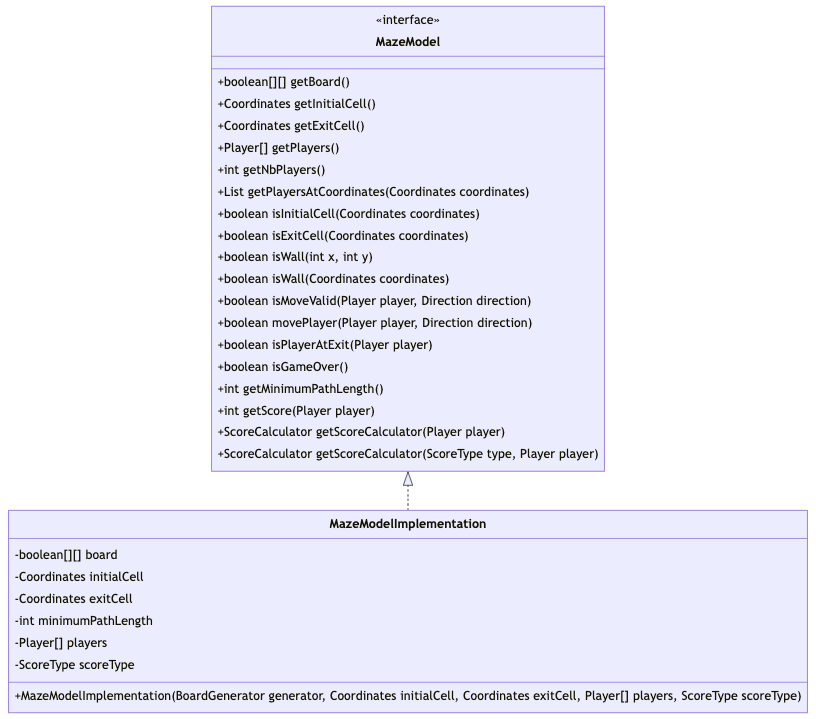
\includegraphics[width=15cm]{ressources/Implementation/Labyrinthe/Modele/MazeModelAndImplementation.png}
    \caption{L'interface MazeModel et son implémentation MazeModelImplementation}
    \label{fig:MazeModelAndImplementation}
\end{figure}

Les labyrinthes sont générés grâce à un générateur qui est géré par l'interface
\textbf{\textit{BoardGenerator}}' et son implémentation
'\textbf{\textit{DepthFirstGenerator}}. L'algorithme de génération utilisé est
le Randomized Depth-First Search.

\begin{figure}[htb]
    \centering
    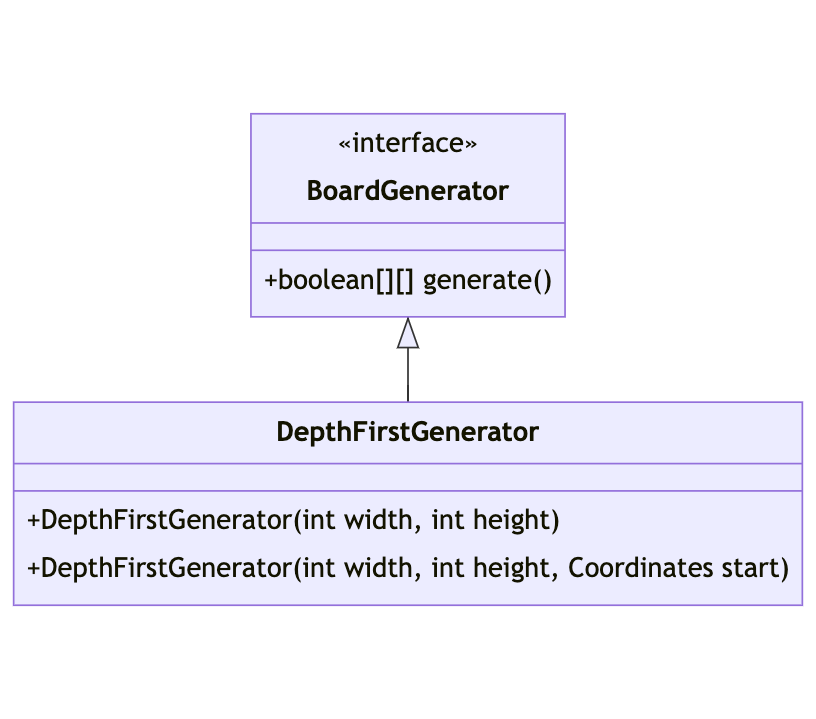
\includegraphics[width=8cm]{ressources/Implementation/Labyrinthe/Modele/DepthFirstGenerator.png}
    \caption{L'interface MazeModel et son implémentation MazeModelImplementation}
    \label{fig:MazeModelAndImplementation}
\end{figure}

L'enum \textbf{\textit{GameMode}} permet de définir les différents modes de
jeu. Chaque type de jeu a sa propre implémentation de l'interface
\textbf{\textit{GameModeData}} qui sert à définir les données des paramètres de
jeu (taille, type de score, difficulté) et la classe \textbf{\textit{GameData}}
se charge de regrouper ces données avec la liste des joueurs.
% TODO: Ajouter une image du diagramme des classes de l'implémentation de l'enum \textbf{\textit{GameMode}}' avec son implémentation '\textbf{\textit{GameModeData}}' et de la case '\textbf{\textit{GameData}}

Les labyrinthes sont créés grâce aux méthodes de la classe
\textbf{\textit{MazeModelFactory}} qui se charge de mettre à disposition des
méthodes qui permettent de créer des labyrinthes de différentes tailles selon
les différents modes de jeu.
% TODO: Ajouter une image du diagramme des classes de l'implémentation de la classe \textbf{\textit{MazeModelFactory}}

En ce qui concerne les joueurs, nous avons une interface
\textbf{\textit{Player}} avec son implémentation
\textbf{\textit{PlayerImplementation}} qui permettent de représenter un joueur.
Ces derniers sont caractérisés par un nom, une couleur, des coordonnées, un
statut, un nombre de mouvements et un temps qui correspond à la durée nécessaire pour
finir le labyrinthe. Ces deux dernières données servent à calculer le score
d'un joueur.
%TODO : Ajouter une image du diagramme des classes de l'implémentation de l'interface \textbf{\textit{Player}}' et de son implémentation '\textbf{\textit{PlayerImplementation}}

Pour pouvoir calculer le score des joueurs, nous avons plusieurs éléments qui
utilisent les données évoquées précédemment. L'interface
\textbf{\textit{ScoreCalculator}} et ses implémentations permettent de calculer
le score d'un joueur à partir d'une implémentation de
\textbf{\textit{ScoreInfo}} qui stocke les informations nécessaires. La classe
\textbf{\textit{ScoreCalculatorFactory}} se charge de créer des instances
d'implémentations de \textbf{\textit{ScoreCalculator}} en fonction du type de
score et des informations selon le type de score (respectivement grâce à l'enum
\textbf{\textit{ScoreType}}, et \textbf{\textit{ScoreInfo}}). Le calcul du
score se fait mathématiquement en fonction du nombre de mouvements, du temps
passé et de la difficulté du labyrinthe.
% TODO : Ajouter une image du diagramme des classes de \textbf{\textit{ScoreCalculator}}' et de ses implémentations, de '\textbf{\textit{ScoreCalculatorFactory}}', de l'enum '\textbf{\textit{ScoreType}}' et de '\textbf{\textit{ScoreInfo}}

L'enum \textbf{\textit{Direction}} permet de définir les quatre directions de
déplacement.
% TODO : Ajouter une image du diagramme des classes de l'enum \textbf{\textit{Direction}}